\documentclass[12pt,a4paper,ngerman]{article}
\usepackage[english]{babel}
\usepackage[latin9]{inputenc}
\usepackage[T1]{fontenc}
\usepackage[left]{eurosym}
\usepackage{amsmath}
\usepackage{amsthm}
\usepackage{ulem}
\usepackage{rotating}
\usepackage{multirow}
\usepackage{listings}
\usepackage{color}
\lstset{numbers=none, numberstyle=\tiny, keywordstyle=\color{blue}, numbersep=5pt, language=SQL, basicstyle=\footnotesize}

% Dokumentinfo
\title{Datenbanken 1\\
       Written report on constructing a simple database system}
\date{\copyright \today}
\author{Michael Hraschan, 0831401 \\
				Achleitner Florian, 0830434\\
				Matthias Viertler, 0830605 \\}

\selectlanguage{english}
%
\begin{document}

\maketitle

\newpage
%
\tableofcontents % if you want
\clearpage
%
\pagestyle{plain}

\section{Database schema}

\begin{figure}[htbp]
	\centering
		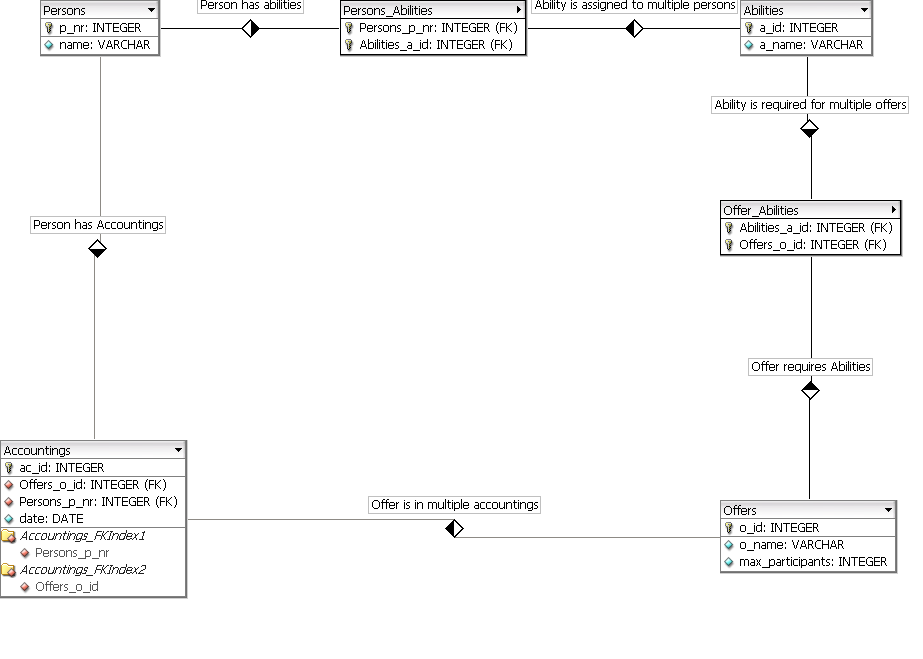
\includegraphics[width=1.00\textwidth]{Images/database_design.png}
	\caption{Scheme of the used database.}
	\label{fig:database_design}
\end{figure}

\begin{itemize}
	\item Domains
		\begin{itemize}
			\item \textbf{p\_nr Integer;} Person number
			\item \textbf{name String;} Person name
			\item \textbf{a\_id Integer;} Ability id
			\item \textbf{a\_name String;} Ability name
			\item \textbf{o\_id Integer;} Offer id
			\item \textbf{o\_name String;} Offer name
			\item \textbf{max\_participants Integer;} Maximal participants for an offer
			\item \textbf{ac\_id Integer;} Accounting id
			\item \textbf{date Date;} Date of the accounting
		\end{itemize}
	\item Relation: Persons(\textbf{\underline{p\_nr}}, name)
	\item Relation: Persons\_Abilities(\textbf{\underline{Persons\_p\_nr, Abilities\_a\_id}})
	\item Relation: Abilities(\textbf{\underline{a\_id}}, a\_name)
	\item Relation: Offer\_Abilities(\textbf{\underline{Abilities\_a\_id, Offers\_o\_id}})
	\item Relation: Offers(\textbf{\underline{o\_id}}, o\_name, max\_participants)
	\item Relation: Accountings(\textbf{\underline{ac\_id}}, date)
\end{itemize}

\section{Functional dependencies}
\begin{itemize}
	\item Relation: Persons(\textbf{\underline{p\_nr}}, name)
		\begin{itemize}
			\item p\_nr $\rightarrow$ name
		\end{itemize}
	\item Relation: Persons\_Abilities(\textbf{\underline{Persons\_p\_nr, Abilities\_a\_id}})
	\item Relation: Abilities(\textbf{\underline{a\_id}}, a\_name)
		\begin{itemize}
			\item p\_nr $\rightarrow$ a\_name
		\end{itemize}
	\item Relation: Offer\_Abilities(\textbf{\underline{Abilities\_a\_id, Offers\_o\_id}})
	\item Relation: Offers(\textbf{\underline{o\_id}}, o\_name, max\_participants)
		\begin{itemize}
			\item o\_id $\rightarrow$ o\_name
			\item o\_id $\rightarrow$ max\_participants
		\end{itemize}
	\item Relation: Accountings(\textbf{\underline{ac\_id}}, date)
		\begin{itemize}
			\item ac\_id $\rightarrow$ date
		\end{itemize}
\end{itemize}

\section{Normal form}
\subsection{1. normal form}
The table is in the 1. normal form because each table represents a relation and has no repeating groups. 

\subsection{2. normal form}
The table is in the 2. normal form because no non-prime attribute in the tables are funcionally dependent on a part of a candidate key. 

\subsection{3. normal form}
The table is in the 3. normal form because every non-prime attribute is non-transitively dependent on every key of the tables.

\section{A current state of the database}
                        
\begin{table}[h]
	\centering
	\begin{minipage}{0.3\textwidth}
		\begin{tabular}{| c | c |}
			\hline
			\multicolumn{2}{|l|}{\textbf{Persons}} \\ \hline
			\textbf{P\_nr} & \textbf{name} \\ \hline \hline
			1 & Huber											\\ \hline
			2 & Otto											\\ \hline
			3 & Maxmann											\\ \hline
		\end{tabular}
	\end{minipage}\hfill
	\begin{minipage}{0.6\textwidth}
		\begin{tabular}{| c | c |}  
			\hline
			\multicolumn{2}{|l|}{\textbf{Persons\_Abilities}} \\ \hline
			\textbf{Persons\_p\_nr} & \textbf{Abilities\_a\_id}               \\ \hline \hline
			1 & 4											\\ \hline
			2 & 3											\\ \hline
		\end{tabular}
	\end{minipage}
\end{table}

\begin{table}[h]
	\centering
	\begin{minipage}{0.3\textwidth}
		\begin{tabular}{| c | c |} 
			\hline
			\multicolumn{2}{|l|}{\textbf{Abilities}} \\ \hline
			\textbf{a\_id} & \textbf{a\_name}              \\ \hline \hline
			3 & fliegen											\\ \hline
			4 & tauchen											\\ \hline
		\end{tabular}
	\end{minipage}
	\begin{minipage}{0.6\textwidth}
		\begin{tabular}{| c | c | c | c |} 
			\hline
			\multicolumn{4}{|l|}{\textbf{Accountings}} \\ \hline
			\textbf{ac\_id} & \textbf{Offers\_o\_id} & \textbf{Persons\_p\_nr} & \textbf{date}            \\ \hline \hline
			1 & 3 & 1 & 2009-11-24											\\ \hline
			2 & 3 & 3 & 2009-11-24											\\ \hline
			3 & 2 & 3 & 2010-04-23											\\ \hline
		\end{tabular}
	\end{minipage}
\end{table}

\begin{table}[h]
	\centering
	\begin{tabular}{| c | c | c |}
		\hline
		\multicolumn{3}{|l|}{\textbf{Offers}} \\ \hline
		\textbf{o\_id} & \textbf{o\_name} & \textbf{max\_participants} \\ \hline \hline
		1 & flug\_ryanair & 120											\\ \hline
		2 & tauchgang\_malediven & 10											\\ \hline
		3 & Surfing & 100											\\ \hline
		4 & skydiving & 6											\\ \hline
		5 & BASE-jumping & 200											\\ \hline
	\end{tabular}
\end{table}

\begin{table}[h]
	\centering
	\begin{tabular}{| c | c |}
		\hline
		\multicolumn{2}{|l|}{\textbf{Offer\_Abilities}} \\ \hline
		Abilities\_a\_id & Offers\_o\_id               \\ \hline \hline
		3 & 1											\\ \hline
		3 & 4											\\ \hline
		4 & 2											\\ \hline
	\end{tabular}
\end{table}

\newpage

\section{Queries}
\subsection{Relational Algebra}
This query gets all accountings for each person. The query illustrates the join, select and set (join requires is a serie of select and set) operation:
\begin{gather}
Persons \bowtie{}_{}Accountings := \nonumber \\ 
\left\{ p \cup a | p \in Persons \wedge a \in Accountings \wedge p_{[p\_nr]} = a_{[Persons\_p\_nr]} \right\}
\end{gather}
The next query demonstrates the project operation by selecting only the name of the persons table:
\begin{equation}
\pi{}_{name}(Persons) := \left\{ t_{name} | t \in Persons \right\}
\end{equation}
The next query demonstrates the divide operation. Due to the database scheme an additional 'temporary' table is used to demonstrate the divide operation. This table is shown in table~\ref{tbl:temp}. The query itself lists all offers which have only an maximum participant capacity of 80, 100 or 120:
\begin{gather}
	Offers \div Temp := \nonumber \\
	\pi_{Offers'}(Offers) - \pi_{Offers'}((\pi_{Offers'} \times Temp)-Offers)
\end{gather}

\begin{table}[h]
	\centering
	\begin{tabular}{| c | c |}
		\hline
		\multicolumn{1}{|l|}{\textbf{Temp}} \\ \hline
		\textbf{max\_participants}               \\ \hline \hline
		80											\\ \hline
		100											\\ \hline
		120											\\ \hline
	\end{tabular}
	\caption{Temporary table to demonstrate the divide operation. \label{tbl:temp}}
\end{table}

\subsection{Relational Calculus}
\subsubsection{Domain Variables}
The following query gets all abilities for the person 'Otto':
\begin{gather}
\{ p\_nr, p\_name, a\_id, a\_name | \nonumber \\
Persons(p\_nr, p\_name) \wedge Persons\_Abilities(p\_nr, a\_id) \wedge \nonumber \\
Abilities(a\_id, a\_name) \wedge x = 'Otto' \}
\end{gather}
The next query gets all abilities required for for the offer 'Surfing':
\begin{gather}
\{ o\_id, o\_name, a\_id, a\_name | \nonumber \\
Offers(o\_id, o\_name) \wedge Offer\_Abilities(a\_id, o\_id) \wedge \nonumber \\ 
Abilities(a\_id, a\_name) \wedge o\_name = 'Surfing' \}
\end{gather}

\subsubsection{Tuple Variables}
The following query gets all accountings for the person 'Otto', the date for the accounting and the name of the offers:
\begin{gather}
\{ p.name, a.date, o.name | \nonumber \\
Persons(p) \wedge \exists a(Accountings(a) \wedge Offer(o) \nonumber \\
 \wedge p.p\_nr = a.Persons\_p\_nr \wedge a.Offers\_o\_id = o.o\_id) \}
\end{gather}

\subsection{SQL}
The following query selects all abilities for the person 'Otto'. The result of the querie with the current database state is in table ~\ref{tab:sql1}.
\lstinputlisting{query1.sql}

\begin{table}[htbp]
\begin{center}\hspace*{-1,5cm}
\begin{tabular}
{| c | c |}
\hline
name & a\_name                      \\ \hline \hline
Otto & fliegen											\\ \hline

\end{tabular}
\caption{Resulttable of first sql query.\label{tab:sql1}}
\end{center}
\end{table}

The next query selects all persons which have an accouting on the 24.11.2009 for the offer 'Surfing'. The result of the query is in table ~\ref{tab:sql2}.
\lstinputlisting{query2.sql}

\begin{table}[htbp]
\begin{center}\hspace*{-1,5cm}
\begin{tabular}
{| c |}
\hline
name \\ \hline \hline
Huber                      \\ \hline
Maxmann 										\\ \hline
\end{tabular}
\caption{Resulttable of second sql query.\label{tab:sql2}}
\end{center}
\end{table}

The last query selects all available offers which allow more than 10 participants for the person 'Otto' (all offers for which 'Otto' has the required abilities). The result of the query is in table~\ref{tab:sql3}.
\lstinputlisting{query3.sql}

\begin{table}[htbp]
\begin{center}\hspace*{-1,5cm}
\begin{tabular}
{| c | c |}
\hline
o\_name & max\_participants                      \\ \hline \hline
flug\_ryanair & 120											\\ \hline

\end{tabular}
\caption{Resulttable of third sql query.\label{tab:sql3}}
\end{center}
\end{table}

\section{Practical implementation of the database with mySQL}
These queries generate the tables in the current database.
\lstinputlisting{tables.sql}

Insert some sample data into the above created tables.
\lstinputlisting{values.sql}

\end{document}
